\section{Background}

The ultimate assessment standard for knowledge is its ability to inform action.
As such, neuroscience incrementally aims to support the development of meaningful and predictable control of the brain.
Within this endeavour, it is the most easily accessible components of the brain, given current technology, which can provide the greatest opportunities for advancement.

The dopaminergic system is an evolutionarily well-conserved \cite{Yamamoto2011}, strongly localized, and widely projecting set of neurons (\cref{fig:ml}).
On account of their small number, tractography commonly fails to resolve the degree centrality of the dopaminergic system, and thus it is not commonly depicted as a significant network node.
However, it is precisely the small number of widely branching and closely similar neurons, which makes the dopaminergic system a credible candidate for truly node-like function in coordinating brain activity.
As is expected given such salient features, the system is widely implicated in neuropsychiatric phenomena (including
addiction \cite{DiChiara1988,DiChiara1999},
attentional control \cite{Nieoullon2002},
motivation \cite{Salamone1994},
creativity \cite{Chermahini2010},
personality \cite{Depue1999},
neurodegeneration \cite{Masliah2000},
and schizophrenia \cite{Howes2009}),
and is a common target for pharmacological interventions.
Manipulation of the dopaminergic system extends widely beyond the medical field, and includes performance-enhancing \cite{Mehta2000,Turner2003}, as well as recreational usage \cite{DiChiara1988}.
As such, better and more predictively powerful models of the dopaminergic system can enhance numerous aspects of human activity, in the clinic and beyond.

\begin{sansmath}
\begin{figure*}[h!]
	\centering
	\hspace*{\fill}
	\begin{subfigure}{.527\textwidth}
		\centering
		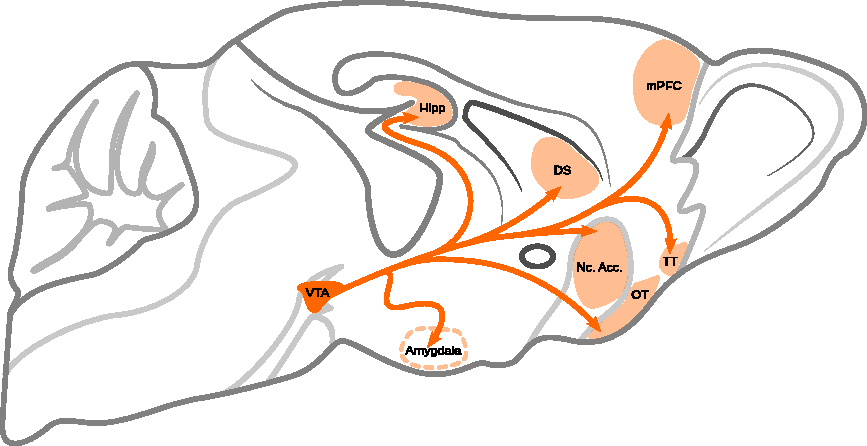
\includegraphics[width=\textwidth]{img/model_literature}
		\caption{
			Literature-based schematic map of VTA dopaminergic projections \cite{Aransay2015,Fields2007,Ikemoto2007,Hnasko2012,Pan2010}.
			Dotted structures are off-slice, and projection arrows do not reflect fiber bundle paths.
			Abbreviations: Hipp (Hippocampus), DS (Dorsal Striatum), NAcc (Nucleus Accumbens), OT (Olfactory Tuberculum), mPFC (medial Prefrontal Cortex), TT (Tenia Tecta).
			}
		\label{fig:ml}
	\end{subfigure}\hfill
	\begin{subfigure}{.44\textwidth}
		\centering
		\vspace{-1em}
		\includedot[width=1.1\textwidth]{data/network_model}
		\vspace{-0.6em}
		\caption{
			Simplified network model of 1-step signal relay following optogenetic stimulation of the VTA.
			The $\mathrm{u_1}$ weighting corresponds to VTA somatic excitability and $\mathrm{u_{2a},u_{2b},u_{2c}}$ and $\mathrm{u_{2d}}$ correspond to transmission at the dopaminergic synapses in the respective projection areas.
			}
		\label{fig:nm}
	\end{subfigure}
	\hspace*{\fill}
	\begin{subfigure}{.985\textwidth}
		\centering
		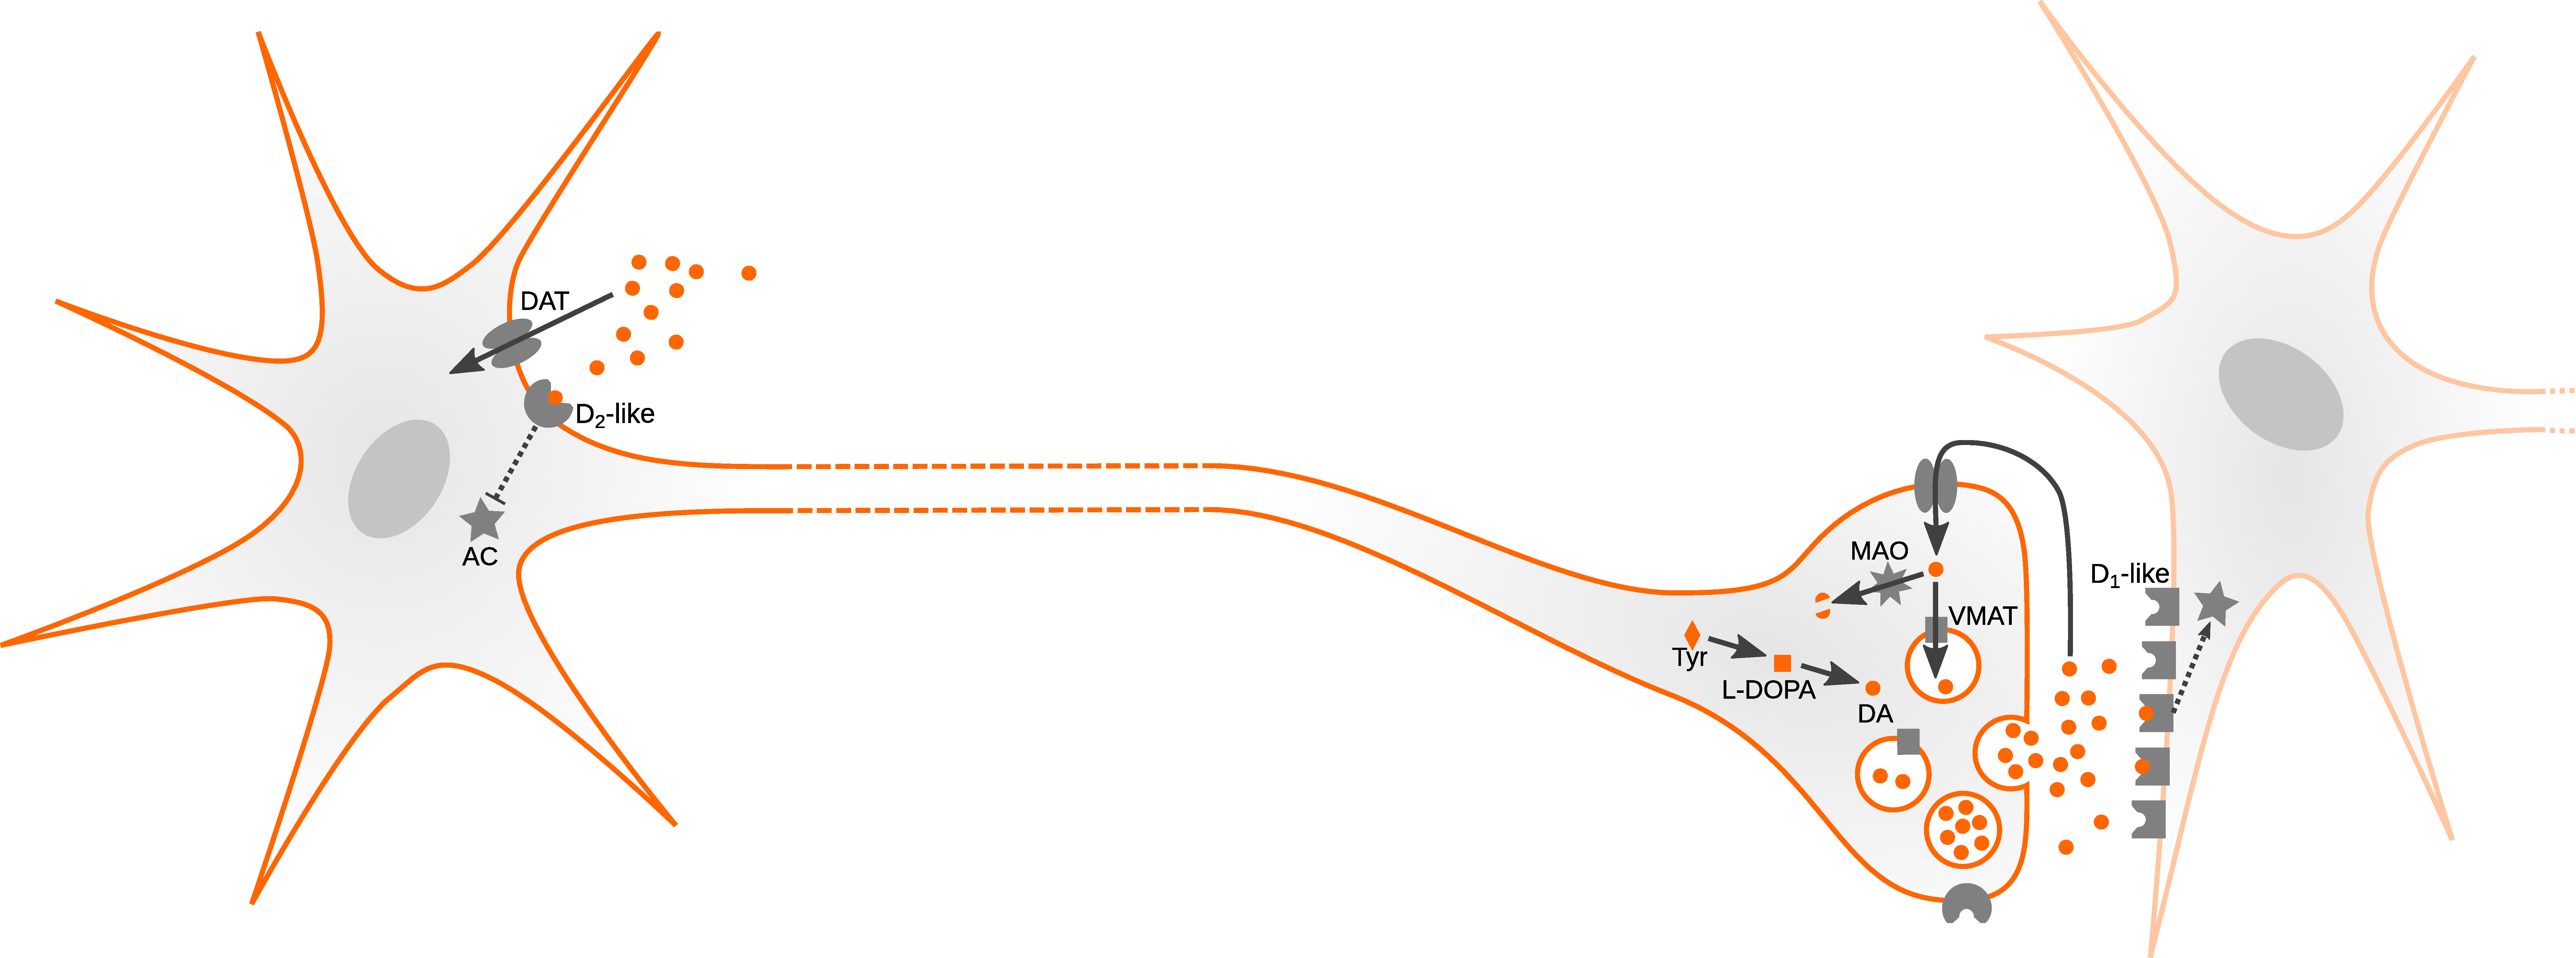
\includegraphics[width=\textwidth]{img/da}
		\caption{
			Schematic overview, which can be applied to model the dopaminergic neurons of the VTA.
			Due to the projection distance and the manifold projection areas the soma is located in the VTA, and the synapses in one or multiple other voxels in the projection areas.
			Excitability at the soma are contingent on $\mathrm{D_2}$ autoinhibition, while transmission at the synapse is contingent on dopamine metabolism, turnover, and postsynaptic $\mathrm{D_1}$ expression.
			Abbreviations: AC (adenylyl cyclase), DA (dopamine), DAT (dopamine transporter), MAO (monoamine oxydase), VMAT (vesicular monoamine transporter), Tyr (tyrosine) \cite{Torres2003}.
			}
		\label{fig:cm}
	\end{subfigure}
	\caption{
		\textbf{The cell biological compartmentalization of dopaminergic neurotransmission (and susceptibility to psychopharmacology) can partly be mapped onto neuroanatomical features by a simple network model.}
		Depicted are schematic overviews of the VTA dopaminergic system at various spatial resolutions.
		}
	\label{fig:m}
\end{figure*}
\end{sansmath}

Neuroscience experimentation in human subjects is methodologically constrained, and must rely extensively on model animal research for cell biological insights, which are instrumental to the refinement of interventions.
Due to high evolutionary conservation, however, the dopaminergic system is an excellent candidate for translational study.
Of the common model animals, the mouse offers advantages not only absent from higher primates, but from most other model animals in general.
These include short generation spans, broad availability of transgenic lines, highly accessible histology, and the smallest size among mammalian model organisms.
Far from trivial, this latter trait offers a significant advantage for numerous imaging techniques, including optics, optoacoustics, and magnetic resonance imaging (MRI).
Furthermore, the small size greatly increases experiment scalability and multi-center reproducibility.
Of particular relevance to pharmacological research, the mouse possesses a high metabolic rate, allowing for rapid drug clearance and thus high contrast in repeated drug administrations blocks.

As it coordinates phenomena such as perception, decision, and action, the function of the brain is highly holistic.
Consequently, localized study of the brain only offers limited insight into the etiology of these phenomena, just as localized manipulations of the brain only offer very limited control over its function.
This consideration not only recommends the study of widely projecting neurotransmitter systems, but also suggests that whole-brain measurement techniques are uniquely suited to describe them.
Owing to its deep penetration, high rostrocaudal coverage, and large-scale usage in human studies, functional MRI (fMRI) is thus one of the foremost methods for studying how the dopaminergic system modulates brain function.

Imaging a neurotransmitter system comprised of a small number of cells, based only on endogenous signalling, is highly unreliable due to a very low signal to noise ratio (SNR).
This issue can, however, be surmounted by introducing exogenous signal, via stimulation.
While the colocalization of widely projecting dopaminergic cell bodies into nuclei makes targeting comparatively easy, dopaminergic nuclei also contain notable populations of non-dopaminergic cells.
Activating such cells may confound dopaminergic function, as they have different projections and pharmacological susceptibilities \cite{Taylor2014}.
In order to specifically target dopaminergic cells, they need to be sensitized to an otherwise inert stimulus in a transcription-dependent manner.
This can be achieved via optogenetics, a method based on light-stimulation of cells expressing a light-sensitive transmembrane protein \cite{Boyden2005}.
Cell-type selectivity can be produced by Cre-conditional channelrhodopsin vector delivery \cite{Orban1992} to transgenic animals expressing Cre-recombinase under a dopaminergic promoter.
Following protein expression, stimulation can be delivered via an implanted optic fiber.
The combination of this stimulation method with fMRI is commonly referred to as opto-fMRI \cite{Desai2011,Grandjean2019}.

In the interest of developing a powerful dopaminergic opto-fMRI assay with maximal brain coverage, optogenetic stimulation is best leveraged by selecting a stimulation site with the highest number of dopaminergic projections.
While the dopaminergic system is centralized in the midbrain, it consists not of one, but of two pairs of lateralized nuclei, the Ventral Tegmental Area (VTA), and Substantia Nigra pars compacta (SNc).
Of these, the VTA has the broader distribution of efferents, whereas the SNc projects primarily to the dorsal striatum \cite{Pan2010}.

The most popular means of producing spatially resolved sensitivity summaries from fMRI, and opto-fMRI in particular, is general linear modelling (GLM) of stimulus evoked activity \cite{Friston1995}.
For this purpose, a precisely specified stimulus train is presented to the brain, and convolved with an impulse response function (IRF) for analysis.
Subsequently, a mass univariate regression analysis is performed across all voxels, allowing them to be assigned parameter values, which denote the strength of activation, as adjusted for the sample noise.
While powerful, this approach is also strongly limiting, since it implies that all voxels in the brain are exposed in an indistinguishable fashion to the stimulation.
Particularly in cases where stimulation is introduced via well-known pathways, a simple network model for signal transmission can easily be implemented via seed-based connectivity (\cref{fig:nm}).
Additionally, in the case of neurotransmitter systems with colocalized cell bodies and long efferent projections, the macroscopic resolution of fMRI can be used to distinguish cell biological processes.
This is done by mapping somatodendritic processes (e.g. excitability upon depolarization at the soma) to “cell-body“ voxels, the and signal transmission at the synapse to “projection“ voxels (\cref{fig:cm}).

To enable the whole-brain modelling of human VTA dopaminergic function in mice, three novel research outputs need to be produced.
Firstly, a proof-of-principle study needs to be conducted and a dataset published, which documents the feasibility of dopaminergic VTA opto-fMRI in the mouse.
The study design needs to include controlled but significant methodological variation, in order to lay a reliable and well-informed foundation for the technique.
Secondly, parameter variation effects need to be described and evaluated, to ascertain what conclusions pertaining to dopaminergic function can already be drawn, and in how far the method can be re-used as a system assay.
Lastly, a voxelwise summary of baseline dopaminergic function needs to be published in a standard volumetric space, to easily enable co-registration, result integration, and result comparison.
